


Studies of transcriptome dynamics provide a basis for understanding functional elements of the genome and the complexity of gene regulation.
The dengue vector mosquito, \Aea, exhibits great adaptability to diverse ecological conditions, is phenotypically polymorphic, and shows variation in vectorial capacity to arboviruses.
Previous genome sequencing showed richness in repetitive DNA and transposable elements that can contribute to genome plasticity.
Population genetic studies revealed a varying degree of worldwide genetic polymorphism.
However, the extent of functional genetic polymorphism across strains is unknown.
The transcriptomes of three \Aa\ strains, \gls{CTM}, \gls{Rex-D} and \gls{LVP}, were compared.
CTM is more susceptible than \gls{Rex-D} to infection by dengue virus serotype 2.
A total of 4188 transcripts exhibit either no or small variation (< 2-fold) among sugarfed samples of the three strains and between sugarfed and bloodfed samples within each strain, corresponding most likely to genes encoding products necessary for vital functions.
Transcripts enriched in bloodfed mosquitoes encode proteins associated with catalytic activities, molecular transport, metabolism of lipids, carbohydrates and amino acids, and functions related to blood digestion and the progression of the gonotropic cycle.
Significant qualitative and quantitative differences were found in individual transcripts among strains including differential representation of paralogous gene products.
The majority of immunity-associated transcripts decreased in accumulation after a bloodmeal and the results are discussed in relation to the different susceptibility of \gls{CTM} and \gls{Rex-D} mosquitoes to \gls{DENV2} infection.

This mosquito species is phenotypically polymorphic, has great adaptability to diverse ecological conditions, and shows variation in vectorial capacity for arboviruses \cite{Bennett2002,Black2002,Kuno2010}.
Genetic polymorphism among geographically distinct \Aa\ populations is documented \cite{Urdaneta-Marquez2011}; however, the extent of genome sequence polymorphism and its effects on transcriptional activity are not known.

The transcriptional profiles of three \Aa\ strains, \gls{LVP}, \gls{CTM}, \gls{Rex-D}, were investigated.
\gls{LVP} originated in West Africa in the 1930s, and its genome is sequenced \cite{Nene2007}, \gls{CTM} was derived from the Yucatan Peninsula in Mexico in the early 2000s \cite{Bennett2002,Gubler1985,Richardson2006a}, whereas \gls{Rex-D} was established from mosquitoes captured in Puerto Rico in the early 1990s \cite{Miller1991}.
\gls{CTM} supports a faster and more intense dissemination of \gls{DENV2} than \gls{Rex-D} \cite{Bennett2002,Salazar2007}.
Our data show significant differences in transcript accumulation among strains, and the results may account for the differing susceptibility of \gls{CTM} and \gls{Rex-D} mosquitoes to virus infection.


\subsection{Results}
\subsubsection{RNA-seq mapping summary}

Transcriptional profiles of \gls{LVP}, \gls{CTM}, and \gls{Rex-D} strains before and after a bloodmeal were compared.
RNA-seq libraries were generated with the use of RNA extracted from females collected 3 to 5 days after eclosion and kept either on a sugar diet (S) or harvested 5 h \gls{PBM} (B) (not shown).
Two RNA-seq libraries were constructed for each RNA sample.
The reproducibility of the parallel libraries was verified (not shown), and the data from the two technical replicates were merged for further analyses.
Reads mapping to multiple genomic locations were discarded during Bowtie alignment \cite{Langmead2009}.
As a consequence, the accumulation levels of transcripts encoded by highly conserved gene families are under-estimated.
This bias is expected to affect all samples equally; therefore, if the absolute accumulation level of a transcript is underestimated, differences across conditions still can be calculated.



\subsubsection{Constitutively accumulated transcripts}

A total of 4188 transcripts exhibit no or small variation (≤ 2-fold) among S samples of the three strains and between B and S samples within each strain and correspond most likely to genes that encode products necessary for vital and/or basal metabolic functions (not shown).
Function−parent attributions for this group of transcripts revealed a predominance of those encoding proteins with binding activity over transcripts with molecular function and catalytic activity (not shown).
Functional description is available for 2262 of these 4188 transcripts \cite{Lawson2009} (not shown).
More than 10 transcripts were found associated with each of the following classes: protein recycling (ubiquitin and proteasome), zinc finger proteins, WD-repeat proteins associated with diverse functions (i.e. RNA-processing complexes, transcription, cytoskeleton assembly), ribosome proteins, signal transduction (GTP binding proteins, G coupled proteins), redox processes (cytochrome), translation (eukaryotic translation initiation factor), transcription (transcription factors, mediator complex), membrane trafficking (rab), cell growth, differentiation and survival (ras), and immunity (PIWIs, autophagy proteins, galectins, TOLL, IMD, and JACK-STAT pathway signaling members).


Approximately 25\% of all analyzed transcripts accumulated differentially in S mosquitoes of different strains.
However, in the majority of cases the differences observed were lower than 2-fold (not shown).
Here is described only differences between the DEN-refractory \gls{Rex-D} and the more permissive \gls{CTM} strain.
Totals of 2992 and 2080 transcripts accumulated more in \gls{Rex-D} or \gls{CTM}, respectively.
Six were accumulated more than 5-fold in \gls{CTM} with respect to \gls{Rex-D}, including four of unknown function, one (AAEL005534-RA) annotated as a gonadotropin-inducible transcription factor, and one (AAEL014188-RA) annotated as a serine-type endopeptidase.
In contrast, 310 transcripts accumulated ≥ 5-fold in \gls{Rex-D} with respect to \gls{CTM}.
Functions could be attributed to 51\% of these and they include aldehyde oxidases, cytochrome P450s, G-coupled receptors, N-acetylgalactosaminyltransferases, and nicotinic acetylcholine receptors.
Immunity-associated transcripts accumulated differently in \gls{CTM} and \gls{Rex-D} S mosquitoes include five C-type lectins (AAEL008681-RA [CTL12], AAEL012353-RA [CTL15], AAEL005482-RA [CTL18], AAEL013566-RB [CTLGA2], AAEL017484-RA [CTLGA4]), two heme peroxidases (AAEL00376-RA [HPX4], AAEL002354-RA), one class B scavenger receptor (AAEL010655-RA [SCRBSP2]), a fibrinogen-related protein (AAEL008646-RA [FREP10]), and a Toll-like receptor (AAEL000671-RA [TOLL6]).


Quantitative reverse transcriptase, gene amplification, i.e., polymerase chain reaction (qRT-PCR) was performed on a selection of 13 transcripts and RNA from \gls{CTM}, \gls{Rex-D}, and \gls{LVP} mosquitoes.
The qRT-PCR results validated the RNA-seq data, with only two exceptions (transcript AAEL011871-RA in \gls{CTM} and AAEL008848-RA in \gls{Rex-D}; not shown).
To assess the similarity of the RNA-seq data with the qRT-PCR measurements, we calculated Pearson correlations of 0.97 (p < 0.001), 0.85 (p < 0.001), and 0.90 (p < 0.01) for \gls{LVP}, \gls{CTM}, and \gls{Rex-D}, respectively.
T-test values were 2.18 (p = 0.148), 2.18 (p = 0.453), and 2.18 (p = 0.188), respectively, for the three strains (not shown).

The accumulation of 1845 and 981 transcripts consistently increased and decreased, respectively, in all three strains after a bloodmeal (not shown).
In general, \gls{Rex-D} exhibited the lowest fold-changes and the smallest number of transcripts accumulated highly after the bloodmeal (not shown).
This observation supports the interpretation that \gls{CTM} mosquitoes respond quicker or more intensively to a bloodmeal than \gls{LVP} and \gls{Rex-D}.
To test this hypothesis, the expression profiles of five transcripts were analyzed by qRT-PCR at 5, 8, 12, and 24 h \gls{PBM}.
Results for four of the five transcripts tested showed a greater response of \gls{CTM} to a bloodmeal compared with mosquitoes of the other two strains (not shown).




Despite the observation that the same functional classes are represented within groups of transcripts that increased and decreased in accumulation after a bloodmeal, the numbers of transcripts associated with the various functions differed significantly (not shown).
The transcripts accumulated after a bloodmeal were enriched in functions related to protein-turnover and chaperones, transcription, translation, posttranslational modification, and RNA processing.
These transcripts encode proteins associated with catalytic activities, in transport and metabolism of lipids, carbohydrates and amino acids, and related to blood digestion and the progression of the gonotropic cycle.
Many of the transcripts showing the greatest decrease in accumulation after a bloodmeal in all three strains encode structural proteins.

The number of strain-specific transcripts varying highly (< 10-fold) in abundance between B and S mosquitoes is smaller in general than those found in all three strains (not shown).
\gls{CTM} mosquitoes show both the greatest number of strain-specific, differentially accumulated transcripts (not shown) and the largest range of changes in transcript accumulation levels.
Overall, the largest proportion of transcripts showing strain-specific increased accumulation after bloodmeal are linked to binding and catalytic functions and associated with transcription, translation, and posttranslational modification, whereas the largest proportion of strain-specific decreased transcripts are linked to transcription, translation, posttranscriptional modification, and RNA processing in \gls{LVP} and \gls{CTM} and to transport and metabolism of lipids, carbohydrates, and amino acids in \gls{Rex-D} (not shown).


\subsubsection{Protein network analysis of bloodmeal-induced changes in transcript accumulation}

By using a Markov Cluster algorithm, \cite{Guo2010} developed a protein interaction network in which 3500 \Aa\ proteins are organized into 494 functional modules.
A total of 2465 of these proteins are encoded by transcripts exhibiting significant differential accumulation between B and S mosquitoes in at least one of the three strains analyzed (not shown).
Modules enriched in Gene Ontology terms for cytoplasm organization and biogenesis, ribosome biogenesis and assembly, transcription, DNA metabolic processes, response to endogenous stimuli, and cell cycle were enriched significantly with proteins encoded by transcripts increased in accumulation in all three strains after a bloodmeal (not shown).
A module enriched in Gene Ontology terms for cytoskeleton organization and biogenesis, reproduction, and cell differentiation was enriched significantly with proteins corresponding to transcripts consistently decreased in accumulation following a bloodmeal.
Results from the protein network analyses are consistent with those from functional attribution of the differentially accumulated transcripts.

\subsubsection{Metabolic pathways involving transcripts differentially accumulated post-bloodmeal}

\begin{figure}[h]

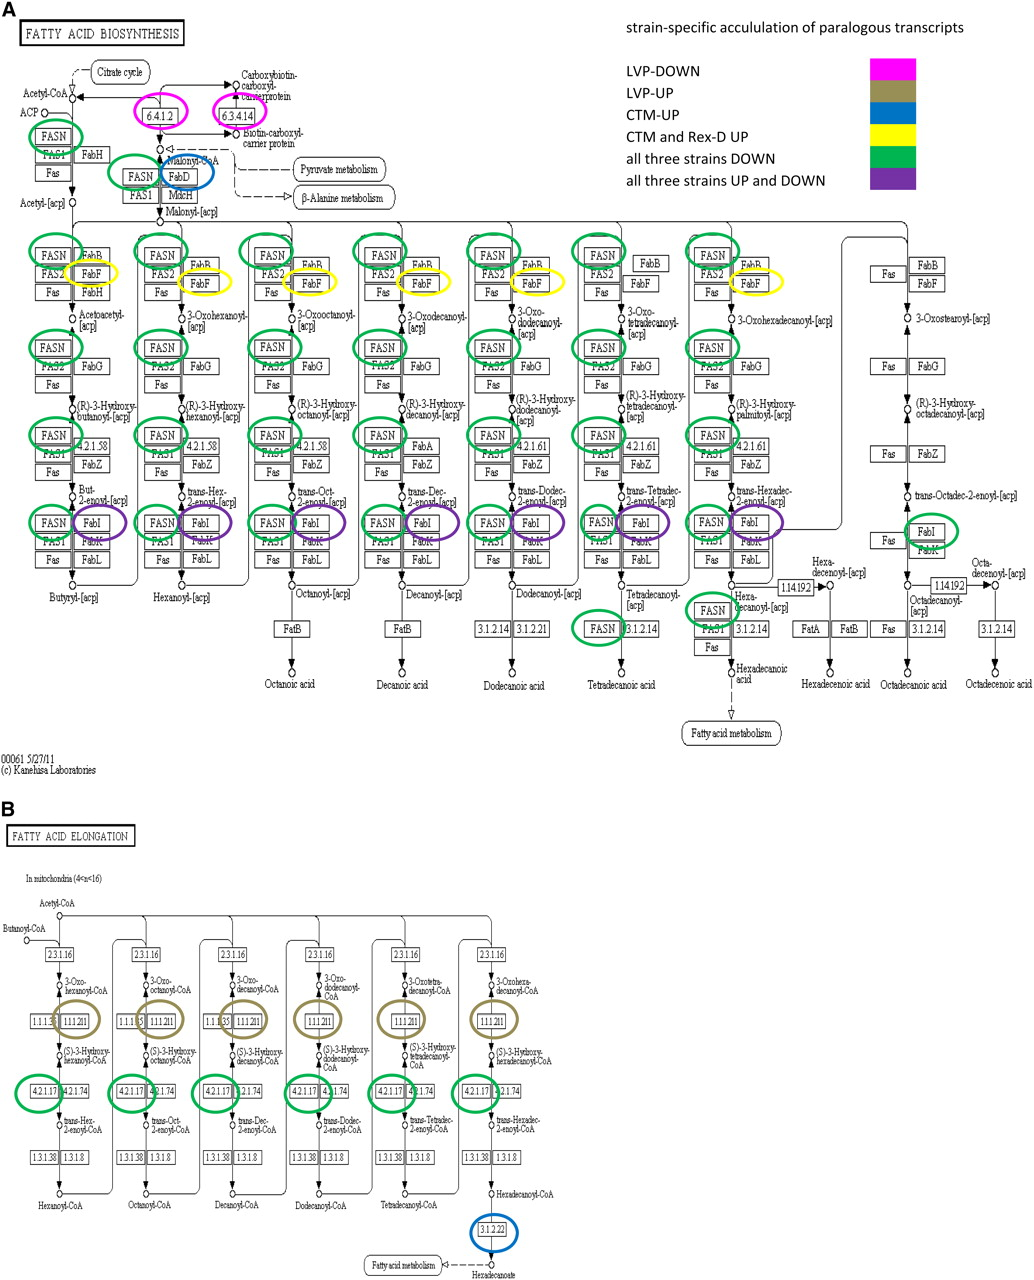
\includegraphics[width=.9\textwidth]{figures/figs/aa-diff-paralogs.jpg}

\caption[Fatty acid biosynthesis and elongation in mitochondria]{\sf \textbf{Fatty acid biosynthesis and elongation in mitochondria:} Proteins corresponding to transcripts accumulated in a strain-specific manner are circled in a color corresponding to the strain and condition defined in the legend (panels A and B).

Excerpted from \cite{bonizzoni2012strain}}
\label{fig:aa-diff-paralogs}
\end{figure}

Metabolic pathways correlated with transcripts increased in accumulation after a bloodmeal in all three strains were visualized in LinkinPath \cite{Ingsriswang2011} alongside pathways associated with transcripts accumulated in a strain-specific manner and transcripts decreased in accumulation after a bloodmeal (not shown).
As seen with the function−parent attribution analyses, the transcripts increased and decreased in accumulation are associated with proteins involved in similar pathways.
However, differential expression of paralogous genes among the strains was observed that could account for the intensity and/or the rate of pathway activation/deactivation after a bloodmeal.
For example, biosynthesis of fatty acids associates predominantly with transcripts decreased in accumulation in all three strains after a bloodmeal, but the elongation of fatty acids in mitochondria was exclusively associated with transcripts increased in accumulation (Figure \ref{fig:aa-diff-paralogs}).
Proteins corresponding to transcripts accumulated differentially in a strain-specific manner were identified in both cases, with the same protein function encoded by paralogous transcripts in the different strains.
Examples include FabI (enoyl-[acyl carrier protein] reductase) of the fatty acid biosynthesis pathway linked to transcripts AAEL003961-RA and AAEL002493-RA, which significantly increased in all three strains (fold-changes: 1.4-2.4); AAEL009634-RC and AAEL014840-RA, both of which increased 2-fold in \gls{CTM}; AAEL000705-RA, AAEL000689-RA and AAEL004273-RA, which decreased in \gls{CTM} (fold-changes: 2.5-4.4); AAEL009685-RB, which decreased 5.4-fold in \gls{Rex-D}; and AAEL017302-RA, AAEL007669-RA, AAEL008227-RA, AAEL009625-RA, AAEL013491-RA, AAEL017320-RA, AAEL000690-RA, AAEL002228-RA, AAEL003148-RA, AAEL003183-RA, AAEL010075-RA, AAEL012400-RA, and AAEL008016-RA, which decreased in all three strains, with fold-changes in the range of 0.6-11.3.
All of these transcripts are annotated currently as short-chain and steroid dehydrogenases, oxidoreductases, or fatty acid synthases \cite{Ribeiro-AegyXcel} and match to short-chain dehydrogenases in the PFAM database \cite{Finn2008}, with the exception of AAEL002228-RA, whose best match is ketoacyl synthase.
They all have the PKS\_KR enzymatic domain as a best match in the SMART database \cite{Letunic2009}, except for AAEL012400-RA, which matches the SEP enzymatic domain.
The protein HADHA (4.2.1.17 in the fatty acid elongation pathway), functioning as an aldehyde reductase and enoyl-coA hydratase, is associated with transcripts AAEL010146-RB (annotated as 3-hydroxyacyl-coa dehydrogenase) and increased 2.9-fold in \gls{LVP} and AAEL003993-RA (putative cyclohex-1-ene-1-carboxyl-CoA hydratase), which increased in all three strains with fold-changes ranging between 1.6 and 2.3.


Another example of differential accumulation of transcripts representing paralogous genes is seen in the lipase gene family.
Three genes (AAEL001837, AAEL007055, AAEL14551) of the 72 annotated currently as lipases correspond to transcripts accumulated differentially after a bloodmeal in all three strains (fold-changes: −7.5 to 4.3) and eight to transcripts accumulated differentially in a strain-specific manner.
Two (AAEL002909-RA, AAEL001076-RA) of these latter transcripts were found exclusively in S and one (AAEL006970-RA) only in B \gls{CTM} mosquitoes.
The remaining had fold-changes ranging from −2.2 to 2.6.
No reads were mapped in any sample for 21 lipase genes, which may indicate that they are expressed exclusively in adult males or during pre-adult stages of \Aa\ development.
Alternatively, these predicted genes could be pseudogenes.



\subsection{Discussion}
The results reported here reveal that the transcriptomes of \Aa\ mosquitoes from distinct strains vary significantly in complexity and abundance of specific transcripts.
This variation is evident in non-bloodfed mosquitoes and is enhanced after a bloodmeal.
\gls{CTM} showed a larger number of differentially abundant transcripts after a bloodmeal and a wider range of fold-changes than \gls{Rex-D} and \gls{LVP}.


Transcripts associated with metabolism and transport of lipids, carbohydrate and amino acids, and the progression of the gonotropic cycles were among the most increased in accumulation after bloodmeal.
Transcripts decreased most in accumulation after a bloodmeal are associated with structural components.
Transcripts attributed functions in transcription, translation, and posttranslational protein modification also were highly differentially-accumulated, but many of these show strain-specific regulation.
These observations support the hypothesis that important differences among the strains are conferred by distinct patterns of gene expression, protein synthesis and modifications.
Strain differences also may result from selective expression of paralogous transcripts.


Digestion and immunity share bio-products such as \gls{ROS} \cite{Molina-Cruz2008}, and these processes are linked at the protein network level \cite{Guo2010}.
The majority of immunity-related genes were decreased in accumulation in all three strains after a bloodmeal.
The most pronounced decrease in accumulation was observed for the antimicrobial peptide \gls{AMP} (AAEL003389-RA).
Indeed, all AMPs decreased in accumulation with the exception of CecF (AAEL000625-RA), which significantly increased in accumulation exclusively in \gls{CTM}.
The overall AMP decrease may be associated with an increase in bacterial proliferation observed after a bloodmeal \cite{Oliveira2011}.
The most common midgut bacteria do not show proteolysis activity but are implicated in the lysis of red blood cells, which release hemoglobin \cite{Gaio2011}.
At the same time, hemoglobin negatively affects ROS production in the midgut, which triggers bacteria proliferation \cite{Oliveira2011}.
Although ROS reduction potentially favors DEN infection \cite{Oliveira2011}, bacteria proliferation antagonizes it \cite{Xi2008}.
Antioxidant activity by peroxidase and superoxide-dismutase varied across strains.
\gls{CTM} showed the greatest number of transcripts associated with antioxidant activity accumulated after a bloodmeal among the strains analyzed.
In addition, S \gls{CTM} mosquitoes accumulate greater levels of transcripts associated with antioxidant activity than \gls{Rex-D}.
\gls{CTM} also had the largest number of P450 and glutathione-s transferase transcripts accumulated differentially after a bloodmeal, with increases in accumulation up to 15-fold (AAEL000325-RA).
These results support a model of more intense antioxidant activity in B \gls{CTM} than in \gls{Rex-D}, which may facilitate DENV infection in the former.

Transcripts encoding proteins associated with autophagy, IAPs, IMD pathway, and SRRP members represent immunity genes that showed an exception to the overall decline in corresponding-transcript accumulation after a bloodmeal.
Increases were overall within 2-fold.
A notable exception is the IMD pathway member Caspar1 (AAEL014734-RA) that increased 4.7- to 5.8-fold in all strains.
Caspar is a negative regulator of the IMD pathway \cite{Kim2006caspar}; therefore, its up-regulation is consistent with the observed decrease in accumulation of AMPs.

In summary, the \Aa\ strains analyzed demonstrated variability in their transcriptomes before and after bloodmeal.
Profiles differ in the number of transcripts detected, their level of accumulation in S mosquitoes, and in the changes in accumulation following the ingestion of a bloodmeal.
Although these differences may result from distinct RNA turnover rates among strains, it is most likely a result of differential gene regulation.
These data indicate the need for caution in making generalizations about individual gene expression profiles across different strains of \Aa.
For example, constructs used in genetics-based strategies of vector control would require the previous analyses of cross-strain promoter activity \cite{James2011}.
The differences observed encompass several transcripts associated previously with vectorial capacity to DENV.
Future studies will investigate the transcriptomes of \gls{CTM} and \gls{Rex-D} mosquitoes infected with \gls{DENV2}.
Also, it will be necessary to assess the susceptibility of \gls{CTM} and \gls{Rex-D} to other DENV serotypes to determine whether or how their distinct transcriptional responses to bloodmeals described herein influence vector competence.